\documentclass[10pt,a4paper]{article}
\usepackage[utf8]{inputenc}
\usepackage[spanish]{babel}
\usepackage{graphicx}
\usepackage{amsmath}
\usepackage{cite}
\usepackage[left=2cm,right=2cm,top=2cm,bottom=2cm]{geometry}
\author{Rubén Martín}
\title{La Ruina del Jugador}
\date{}
\begin{document}
\maketitle

\begin{abstract}
Imaginemos la siguiente situación: Un jugador tiene un capital de 20 euros y cada instante de tiempo apuesta un euro al lanzamiento de una moneda, ganando un euro si sale cara y perdiendo el euro apostado si sale cruz. Consideramos la variable aleatoria discreta T que nos indica el instante de tiempo en que el jugador se arruina por primera vez. Deberemos por tanto crear una función en R que permita simular y representar gráficamente la ``ruina del jugador'' y presentar el desarrollo mediante un documento de LaTeX\cite{LaTeX}
\end{abstract}

\tableofcontents

\newpage
\section{La Teoría}
Podemos extraer leyendo el ejercicio, que cada lanzamiento de la moneda se comporta como un $experimento\ Bernouilli$. Este tipo de variables aleatorias\cite{prob} se distribuyen de la siguiente forma:
$$P[X=1]=p\ \ \ \ \ \ \ \ \ \ \ $$
$$P[X=0]=1-p=q$$

Por tanto los lanzamientos consecutivos de la moneda se distribuirán según una $distribuci\acute{o}n\ binomial$:
$$P[X=k]=\binom{n}{k} p^k(1-p)^{n-k}$$

La esperanza de dicha variable, $E[X]=np$, nos indica que si seguimos lanzando la moneda indefinidamente ganaremos  las mismas veces que perderemos. Sin embargo tenemos la posibilidad de perder todo el dinero antes de que esto ocurra.
\newpage
\section{Qué Ocurre}
En la tabla que se muestra a continuación se puede observar el comportamiento del capital del jugador una vez que comienza a jugar.

\begin{center}
\begin{tabular}[t]{c c c}
Lanzamientos totales & Lanzamientos ganados & Capital total\\
\hline
1 & 0 & 19\\
1 & 1 & 21\\
2 & 0 & 18\\
2 & 1 & 20\\
2 & 2 & 22\\
$\vdots$ & $\vdots$ & $\vdots$\\
19 & 0 & 1\\
20 & 0 & 0\\
20 & 20 & 40\\
\end{tabular}
\end{center}
Así, si el jugador tiene la ``mala suerte'' de perder todos los lanzamientos se quedaría sin dinero en el instante 20. Sin embargo, si en ese mismo momento hubiese ganado todos los lanzamientos el jugador tendría 40 euros en su poder.
\newpage
\section{El Problema}
\subsection{Planteamiento}
Para modelizar la situación anteriormente descrita deberemos tener en cuenta:

\begin{itemize}
\item La función tendrá un único argumento, el capital inicial. En el caso explicado es de 20 euros, aunque admitiremos que este puede ser otro valor.
\item La moneda se supone no trucada (probabilidad de cara y cruz idéntica, 1/2)
\item El juego termina en el instante en que el capital de que dispone el jugador es 0 (ruina)
\item La función debe devolver los resultados en un gráfico
\end{itemize}

A continuación se desarrollará paso a paso la creación de la función.

\subsection{Creación de la Moneda}
Para la creación de la moneda usaremos la función ya implementa en R {\tt sample} de la siguiente forma:

\begin{verbatim}
moneda = sample(c(1,-1), 1, prob = c(0.5, 0.5))
\end{verbatim}

Tenemos pues un ``lanzamiento'' con un vector de valores (1,-1) para cara y cruz respectivamente. Ambas posibilidades tienen una probabilidad de ocurrir del 50\%, tal y como se observa en el último argumento.

\subsection{Creación del Bucle Principal}
Una vez que tenemos la moneda pasaremos a esbozar qué es necesario en el interior de la función. Se puede suponer leyendo el enunciado del problema que el jugador sigue realizando lanzamientos de moneda hasta que se queda sin dinero, por lo que nos hace falta un bucle que repita esos lanzamientos hasta que no tenga con qué jugar.

En conclusión: la función tiene que tener un parámetro que sea el dinero con el que parte el jugador y un bucle que modifique el valor de esa cantidad dependiendo de si obtiene cara o cruz.

Decidí utilizar el bucle {\tt while}, ya que no sé el momento exacto en el que el jugador perderá.

\begin{verbatim}
ruinaDelJugador = function(capitalInicial)
{
  while(capitalInicial !=0){
    moneda = sample(c(1,-1),1, replace = TRUE, prob = c(0.5,0.5));
    capitalInicial = capitalInicial + moneda;
  }
}
\end{verbatim}

\subsection{Dónde almacenar los datos}
Para representar los datos hará falta un vector que los almacene. A ese vector lo nombraremos como {\tt resultados}, y varía de la siguiente forma:

\begin{verbatim}
resultados <- c(resultados,capitalInicial)
\end{verbatim}

Pero tiene que tomar un valor inicial, que es:

\begin{verbatim}
resultados <- c(capitalInicial)
\end{verbatim}

Resumiendo lo que llevamos hasta ahora:

\begin{verbatim}
ruinaDelJugador = function(capitalInicial)
{
  resultados <- c(capitalInicial);
  while(capitalInicial !=0){
    moneda = sample(c(1,-1),1, replace = TRUE, prob = c(0.5,0.5));
    capitalInicial = capitalInicial + moneda;
    resultados <- c(resultados,capitalInicial);
  }
}
\end{verbatim}

\subsection{Representación gráfica}
Por último se pide que representemos esos valores. Esto es bastante sencillo puesto que solo es necesario utilizar la función {\tt plot}.

\begin{verbatim}
plot(resultados,type = "l",xlab = "Intentos",ylab = "Capital")
\end{verbatim}

Que añadiéndolo a la función quedaría:

\begin{verbatim}
ruinaDelJugador = function(capitalInicial)
{
  resultados <- c(capitalInicial);
  while(capitalInicial !=0){
    moneda = sample(c(1,-1),1, replace = TRUE, prob = c(0.5,0.5));
    capitalInicial = capitalInicial + moneda;
    resultados <- c(resultados,capitalInicial);
 }
  plot(resultados,type = "l",xlab = "Intentos",ylab = "Capital")
}
\end{verbatim}

\subsection{Últimos ajustes}
Para clarificar aún más la gráfica le añadiremos dos líneas horizontales que señalen el valor del dinero con el que parte el jugador y el valor 0. Para ello utilizaremos la función {\tt abline} de la siguiente forma:

\begin{verbatim}
capitalIn <- capitalInicial;

...

abline(h = capitalIn, lty = 3, col = 4);
abline(h = 0, lty = 3, col = 2);
\end{verbatim}

El valor de {\tt capitalIn} indica el valor que ha introducido el jugador, y debe de escribirse antes de modificar el valor de {\tt capitalInicial} en el bucle {\tt while}.

Del mismo modo añadimos un mensaje que indique en qué momento exacto el jugador pierde todo su dinero utilizando el siguiente código:

\begin{verbatim}
print("El jugador se arruina en el momento: ");
print(length(resultados));
\end{verbatim}
\subsection{Conclusiones}
Para terminar uniremos todo el código utilizado y añadiremos un par de ejemplos con sus respectivas gráficas:

\begin{verbatim}
ruinaDelJugador = function(capitalInicial)
{
 capitalIn <- capitalInicial;
 resultados <- c(capitalInicial);

 while(capitalInicial !=0){
 moneda = sample(c(1,-1),1, replace = TRUE, prob = c(0.5,0.5));
 capitalInicial = capitalInicial + moneda;
 resultados <- c(resultados,capitalInicial);
 }

 plot(resultados,type = "l",xlab = "Intentos",ylab = "Capital")
 abline(h = capitalIn, lty = 3, col = 4)
 abline(h = 0, lty = 3, col = 2)

 print("El jugador se arruina en el momento: ");
 print(length(resultados));
}
\end{verbatim}

\bibliographystyle{acm}
\bibliography{ruina}
\subsection{Ejemplos}

\begin{verbatim}
> ruinaDelJugador(20)
[1] "El jugador se arruina en el momento: "
[1] 8682.
\end{verbatim}
\begin{center}
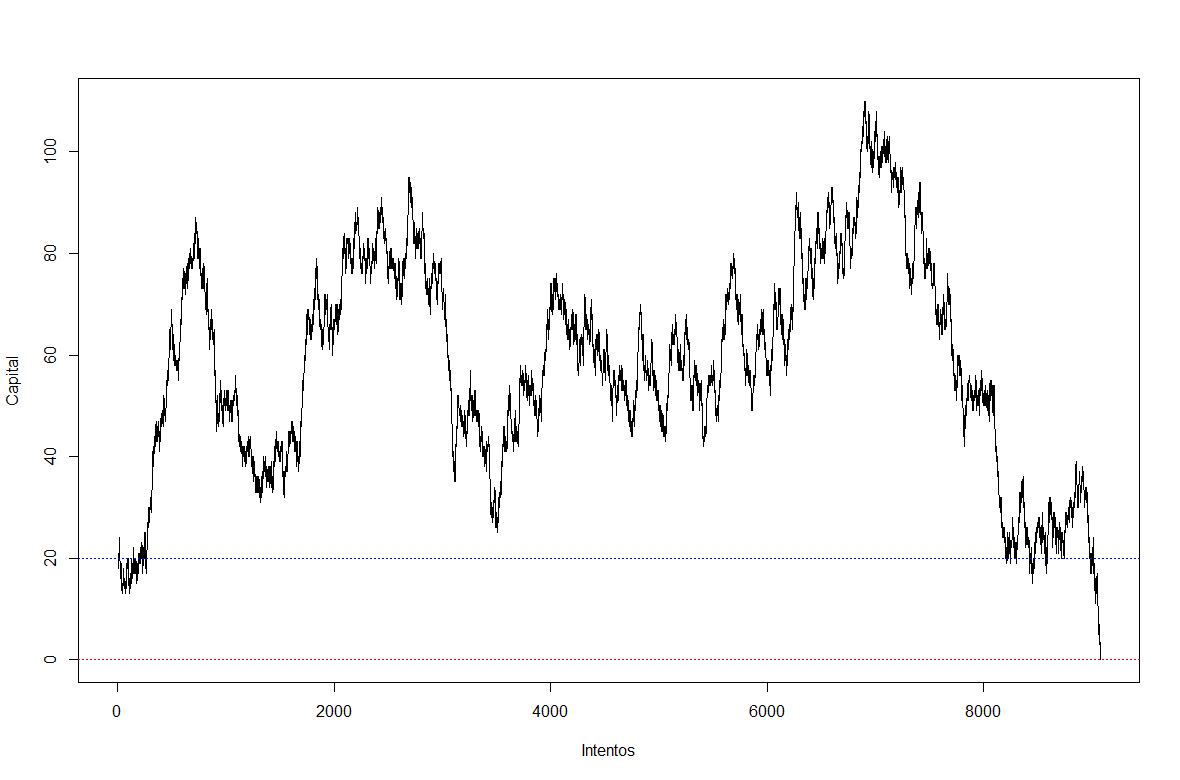
\includegraphics[scale=0.35]{Jugador20_1.png} 
\end{center}


\begin{verbatim}
> ruinaDelJugador(10)
[1] "El jugador se arruina en el momento: "
[1] 482.
\end{verbatim}
\begin{center}
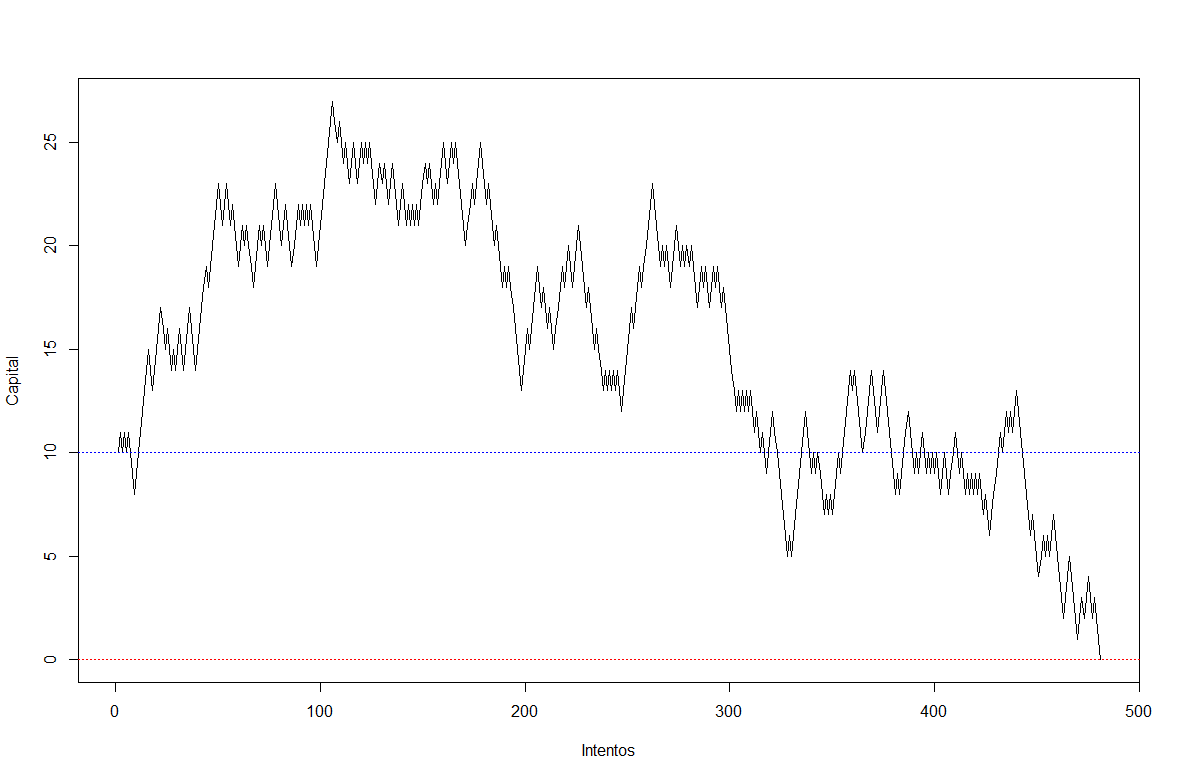
\includegraphics[scale=0.35]{Jugador10_1.png} 
\end{center}

\end{document}
